\documentclass[a4paper,12pt]{report}
\setcounter{secnumdepth}{5}
\setcounter{tocdepth}{3}
\newcounter{ZhRenew}
\setcounter{ZhRenew}{1}
\newcounter{SectionLanguage}
\setcounter{SectionLanguage}{1}
\input{/usr/share/latex-toolkit/template.tex}
\begin{document}
\title{三角學}
\author{沈威宇}
\date{\temtoday}
\titletocdoc
\ch{三角學(Trigonometry)}
\sct{角(Angle)}
\subsection{(平面)角((plane) angle)}
\subsubsection{角度(degree)}
一個完整的圓被平分為 \(360^{\circ}\)。作為單位或省略不寫。物理上無因次。

$'$稱角分,等於六十分之一$^{\circ}$;$''$稱角秒,等於六十分之一$'$。

\[1^{\circ}=60'=3600''\]
\subsubsection{弧度/弳(度)(radian, rad)}
以$r$為半徑的圓的中心為頂點,若展開的角所對應的弧長為$r$,該角的大小就是一弧度。物理上無因次。作為單位或省略不寫。

扇形的弧長等於其弧度乘以半徑;扇形的面積等於其弧度乘以半徑的平方除以二。

\[\frac{1\text{rad}}{1^{\circ}} = \frac{\pi}{180} \approx 57.3 \approx \frac{1}{0.0175} \]
\[\pi\approx 3.14159265,\quad\frac{1}{\pi}\approx 0.3183\]
\sssc{廣義角}
指將角從$[0,2\pi)$擴展到任意實數。
\sssc{同界角}
$\alpha$、$\beta$為同界角$\iff \frac{\alpha -\beta}{2\pi}\in\mathbb{Z}$
\sssc{斜角}
平面上某曲線在某處的斜角指其在該處的切線與$x$軸的最小夾角。一直線之斜角之正切值為其斜率。
\ssc{立體角(Solid angle)}
\sssc{球面度/立弳(steradian, or square radian, sr)}
以$r$為半徑的球的中心為頂點,若展開的立體角所對應的球面表面積為$r^2$,該立體角的大小就是一球面度。物理上無因次。
\subsection{三角測量}
\begin{itemize}
\item \tb{仰角(angle of elevation)}:仰視目標時,視線與水平線的夾角。
\item \tb{俯角(angle of depression)}:俯視目標時,視線與水平線的夾角。
\item \tb{高度角(altitude angle)}:仰視目標時,即仰角;平視目標時,為零;俯視目標時,即負一乘以俯角。
\item \tb{天頂角(zenith angle)/傾(斜)角(inclination)}:90$^{\circ}$減去高度角。
\item \tb{方位角(azimuth or azimuthal angle)}(地理):以正北為0$^\circ$,順時針為正。
\item \tb{象限角(reduced bearing)}(地理):以東南西北某一方位(通常為正北或正南) 為基準,加上向相鄰方位轉向的度數與該相鄰方位,如北35$^\circ$西 代表方位角325$^\circ$、南30$^\circ$西代表方位角210$^\circ$。
\end{itemize}
\ssc{極座標系(Polar Coordinate System)}
極座標系是由一參考點,稱極點(pole)或原點(origin),與一始於極點的射線,稱極軸(polar axis),定義的二維座標系。令一個點在以極點為原點、極軸為$x$軸正向的二維右手笛卡爾座標系中有座標$(r\cos\theta,r\sin\theta)$使得$r\geq 0\land\theta\in[0,2\pi)$,則該點在此極座標系中有極座標$(r;\theta)$,其中$r$稱徑向距離(radial distance or radius),即與原點的距離,$\theta$稱極角(polar angle),即相對於$x$軸、逆時針增加的角位置。
\ssc{球座標系(Spherical Coordinate System)}
\sssc{ISO 80000-2:2019/物理慣例(physics convention)/傾斜角、方位角的球座標系}
ISO 80000-2:2019/物理慣例/傾斜角、方位角的球座標系是由一參考點,稱原點(origin),一始於原點的射線,稱極軸(polar axis),與一包含極軸的平面,稱初始子午面(initial meridian plane),定義的三維座標系。令一個點在以原點為原點、極軸為$z$軸正向、初始子午面為$xz$平面的三維右手笛卡爾座標系中有座標$(r\sin\theta\cos\varphi,r\sin\theta\sin\varphi,r\cos\theta)$使得$r\geq 0\land\theta\in[0,\pi]\land\varphi\in[0,2\pi)$,則該點在此球座標系中有球座標$(r;\theta;\varphi)$,其中$r$稱徑向距離(radial distance or radius),即與原點的距離,$\theta$稱傾(斜)角(inclination)、極角(polar angle)或天頂角(zenith angle),即與$z$軸正向的夾角,$\varphi$稱方位角(azimuth or azimuthal angle),即在$xy$平面正射影相對於$x$軸、逆時針增加的角位置。
\sssc{方位角、高度角的球座標系}
方位角、高度角的球座標系是由一參考點,稱原點(origin),一始於原點的射線,稱極軸(polar axis),與一包含極軸的平面,稱初始子午面(initial meridian plane),定義的三維座標系。令一個點在以原點為原點、極軸為$z$軸正向、初始子午面為$xz$平面的三維右手笛卡爾座標系中有座標$(r\cos\varphi\cos\theta,r\cos\varphi\sin\theta,r\sin\varphi)$使得$r\geq 0\land\theta\in[0,2\pi)\land\varphi\in(-\frac{\pi}{2},\frac{\pi}{2})$,則該點在此球座標系中有球座標$(r;\theta;\varphi)$,其中$r$稱徑向距離(radial distance or radius),即與原點的距離,$\theta$稱方位角(azimuth or azimuthal angle),即在$xy$平面正射影相對於$x$軸、逆時針增加的角位置,$\varphi$稱高度角(altitude angle)或仰角(angle of elevation),即相對於在$xy$平面正射影、逆時針增加的角位置,即$\frac{\pi}{2}$減去高度角。
\sssc{高度角、方位角的球座標系}
高度角、方位角的球座標系是由一參考點,稱原點(origin),一始於原點的射線,稱極軸(polar axis),與一包含極軸的平面,稱初始子午面(initial meridian plane),定義的三維座標系。令一個點在以原點為原點、極軸為$z$軸正向、初始子午面為$xz$平面的三維右手笛卡爾座標系中有座標$(r\cos\theta\cos\varphi,r\cos\theta\sin\varphi,r\sin\theta)$使得$r\geq 0\land\theta\in(-\frac{\pi}{2},\frac{\pi}{2})\land\varphi\in[0,2\pi)$,則該點在此球座標系中有球座標$(r;\theta;\varphi)$,其中$r$稱徑向距離(radial distance or radius),即與原點的距離,$\theta$稱高度角(altitude angle)或仰角(angle of elevation),即相對於在$xy$平面正射影、逆時針增加的角位置,即$\frac{\pi}{2}$減去高度角,$\varphi$稱方位角(azimuth or azimuthal angle),即在$xy$平面正射影相對於$x$軸、逆時針增加的角位置。
\sct{三角比(Trigonometric Ratios)與三角函數(Trigonometric functions)}
\subsection{銳角三角比}
\begin{itemize}
  \item 正弦(Sine,$\sin$):正弦值是對應角的對邊與斜邊之比, 即:\[\sin \theta = \frac{\text{對邊}}{\text{斜邊}}\]
  \item 餘弦(Cosine,$\cos$):餘弦值是對應角的鄰邊與斜邊之比 ,即:\[\cos \theta = \frac{\text{鄰邊}}{\text{斜邊}}\]
  \item 正切(Tangent,$\tan$):正切值是對應角的對邊與鄰邊之比,即:\[\tan \theta = \frac{\text{對邊}}{\text{鄰邊}}\]
  \item 餘切(Cotangent,$\cot$):\[\cot \theta = \frac{1}{\tan \theta}\]
  \item 正割(Secant,$\sec$):\[\sec \theta = \frac{1}{\cos \theta}\]
  \item 餘割(Cosecant,$\csc$):\[\csc \theta = \frac{1}{\sin \theta}\]
\end{itemize}
\subsection{廣義角(General angles)三角比/三角函數幾何定義}
在單位圓中,令角度的測量方式是從正 \(x\) 軸開始,逆時針方向為正角,順時針方向為負角,且角度數值可以是任何實數。任意角度的三角函數值可以表示為:
\begin{itemize}
  \item 正弦(Sine,$\sin$):角 \(\theta\) 的正弦值是單位圓上 對應點的 \(y\) 坐標,即:\[\sin \theta = y\]。為奇函數,定義域$\mathbb{R}$,值域$[-1,1]$,週期$2\pi$,振幅1,線對稱於$x=\qty(n+\frac{1}{2})\pi,n\in\mathbb{Z}$,點對稱於$\qty(\qty(n\pi,n\in\mathbb{Z}),0)$。
  \item 餘弦(Cosine,$\cos$):角 \(\theta\) 的餘弦值是單位圓 上對應點的 \(x\) 坐標,即:\[\cos \theta = x\]。為偶函數,定義 域$\mathbb{R}$,值域$[-1,1]$,週期$2\pi$,振幅1,線對稱於$x=n\pi,n\in\mathbb{Z}$,點對稱於$\qty(\qty(\qty(n+\frac{1}{2})\pi,n\in\mathbb{Z}),0)$,$\cos(x)=\sin\qty(x+\frac{\pi}{2})$ 。
  \item 正切(Tangent,$\tan$):角 \(\theta\) 的正切值是正弦值與餘弦值的比,即:\[\tan \theta = \frac{\sin \theta}{\cos \theta} = \frac{y}{x}\]。為奇函數,定義域$\left\{x\in\mathbb{R}\left |\pi\nmid\qty(x-\frac{\pi}{2})\right.\right\}$,值域$\mathbb{R}$,週期$\pi$,點對稱於$\qty(\qty(\frac{n}{2}\pi,n\in\mathbb{Z}),0)$。
  \item 餘切(Cotangent,$\cot$):\[\cot \theta = \frac{1}{\tan \theta}\]。為奇函數,定義域$\left\{x\in\mathbb{R}\left |\pi\nmid x\right.\right\}$,值域$\mathbb{R}$,週期$\pi$,點對稱於$\qty(\qty(\frac{n}{2}\pi,n\in\mathbb{Z}),0)$,$\cot(x)=-\tan\qty(x+\frac{\pi}{2})$。
  \item 正割(Secant,$\sec$):\[\sec \theta = \frac{1}{\cos \theta}\]。為偶函數,定義域$\left\{x\in\mathbb{R}\left |\pi\nmid\qty(x-\frac{\pi}{2})\right.\right\}$,值域$\left\{y\in\mathbb{R}\left |-1\leq y \lor y\leq 1\right.\right\}$,週期$\pi$,線對稱於$\qty(\qty(n\pi,n\in\mathbb{Z}),0)$,點對稱於$x=\qty(n+\frac{1}{2})\pi,n\in\mathbb{Z}$。
  \item 餘割(Cosecant,$\csc$):\[\csc \theta = \frac{1}{\sin \theta}\]。為奇函數,定義域$\left\{x\in\mathbb{R}\left |\pi\nmid x\right.\right\}$,值域$\left\{y\in\mathbb{R}\left |-1\leq y \lor y\leq 1\right.\right\}$,週期$\pi$,線對稱於$x=\qty(n+\frac{1}{2})\pi,n\in\mathbb{Z}$,點對稱於$\qty(\qty(n\pi,n\in\mathbb{Z}),0)$,$\csc(x)=\sec\qty(x-\frac{\pi}{2})$。
\end{itemize}
\subsection{特殊角三角函數值}
\renewcommand{\arraystretch}{1.5}
\begin{longtable}[c]{|p{0.1\textwidth}|p{0.1\textwidth}|p{0.2\textwidth}|p{0.2\textwidth}|p{0.2\textwidth}|}
\hline
Radian & Angle & $\sin$ & $\cos$ & $\tan$ \\\hline\endhead
0 & 0° & 0 & 1 & 0 \\\hline
$\frac{\pi}{2}$ & 90° & 1 & 0 & \\\hline
$\pi$ & 180° & 0 & -1 & 0 \\\hline
$\frac{3\pi}{2}$ & 270° & -1 & 0 & \\\hline
$\frac{\pi}{4}$ & 45° & $\frac{\sqrt{2}}{2}$ & $\frac{\sqrt{2}}{2}$ & $1$ \\\hline
$\frac{3\pi}{4}$ & 135° & $\frac{\sqrt{2}}{2}$ & $-\frac{\sqrt{2}}{2}$ & -1 \\\hline
$\frac{\pi}{6}$ & 30° & $\frac{1}{2}$ & $\frac{\sqrt{3}}{2}$ & $\frac{\sqrt{3}}{3}$ \\\hline
$\frac{\pi}{3}$ & 60 ° & $\frac{\sqrt{3}}{2}$ & $\frac{1}{2}$ & $\sqrt{3}$ \\\hline
$\frac{2\pi}{3}$ & 120° & $\frac{\sqrt{3}}{2}$ & $-\frac{1}{2}$ & $-\sqrt{3}$ \\\hline
$\frac{5\pi}{6}$ & 150° & $\frac{1}{2}$ & $-\frac{\sqrt{3}}{2}$ & $-\frac{\sqrt{3}}{3}$ \\\hline
$\frac{\pi}{12}$ & 15° & $\frac{\sqrt{6}-\sqrt{2}}{4}$ & $\frac{\sqrt{6}+\sqrt{2}}{4}$ & $2-\sqrt{3}$ \\\hline
$\frac{5\pi}{12}$ & 75° & $\frac{\sqrt{6}+\sqrt{2}}{4}$ & $\frac{\sqrt{6}-\sqrt{2}}{4}$ & $2+\sqrt{3}$ \\\hline
$\frac{\pi}{10}$ & 18° & $\frac{\sqrt{5}-1}{4}$ & $\frac{\sqrt{10+2\sqrt{5}}}{4}$ & $\frac{\sqrt{5}-1}{\sqrt{10+2\sqrt{5}}}$ \\\hline
$\frac{2\pi}{10}$ & 36° & $\frac{\sqrt{10-2\sqrt{5}}}{4}$ & $\frac{\sqrt{5}+1}{4}$ & $\frac{\sqrt{10-2\sqrt{5}}}{\sqrt{5}+1}$ \\\hline
$\frac{3\pi}{10}$ & 54° & $\frac{\sqrt{5}+1}{4}$ & $\frac{\sqrt{10-2\sqrt{5}}}{4}$ & $\frac{\sqrt{5}+1}{\sqrt{10-2\sqrt{5}}}$ \\\hline
$\frac{4\pi}{10}$ & 72° & $\frac{\sqrt{10+2\sqrt{5}}}{4}$ & $\frac{\sqrt{5}-1}{4}$ & $\frac{\sqrt{10+2\sqrt{5}}}{\sqrt{5}-1}$ \\\hline
& 37° & $\approx 0.6018$ & $\approx 0.7986$ & $\approx 0.7536$ \\\hline
& 53° & $\approx 0.7986$ & $\approx 0.6018$ & $\approx 1.3270$ \\\hline
\end{longtable}
\FB
\ssc{三角函數基本關係}
\begin{center}
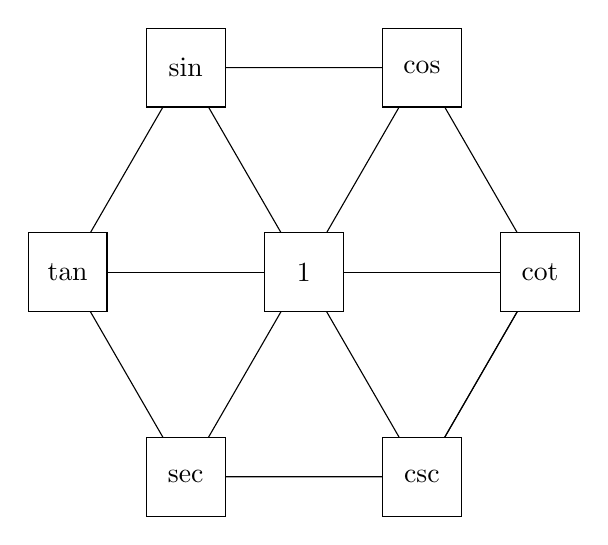
\begin{tikzpicture}
  \foreach \a in {0,60,...,300}
    \node (P\a) at (\a:3) {};
  \draw (P0) -- (P60) -- (P120) -- (P180) -- (P240) -- (P300) -- (P0) -- cycle;
  \draw (P0) -- (P180);
  \draw (P60) -- (P240);
  \draw (P120) -- (P300);
  \draw (P0) -- (P300);
  \node[draw, fill=white, minimum size=1cm, anchor=center] at (P0) {$\cot$};
  \node[draw, fill=white, minimum size=1cm, anchor=center] at (P60) {$\cos$};
  \node[draw, fill=white, minimum size=1cm, anchor=center] at (P120) {$\sin$};
  \node[draw, fill=white, minimum size=1cm, anchor=center] at (P180) {$\tan$};
  \node[draw, fill=white, minimum size=1cm, anchor=center] at (P240) {$\sec$};
  \node[draw, fill=white, minimum size=1cm, anchor=center] at (P300) {$\csc$};
  \node[draw, fill=white, minimum size=1cm, anchor=center] at (0,0) {$1$};
\end{tikzpicture}
\end{center}
\bit
\item 名稱:左側三者為正;右側三者為餘;上面二者為弦;中間二者為切;下面二者為割。
\item 餘角關係:以鉛直軸為對稱軸,位於線對稱位置者為餘角關系,即對於銳角$\theta$,左$(\theta)=$右$\qty(\frac{\pi}{2}-\theta)$。
\item 倒數關係:三條通過中心點的連線為倒數關係,其兩端者互為倒數,相乘為1。
\item 商數關係:六邊形周上,連續三個頂點形成的連線,其兩端者相乘等於中間者。
\item 平方關係:圖中有三個倒正三角形,其在上方兩頂點之二者之平方和等於在下方頂點者。
\eit
\ssc{奇變偶不變,正負看象限}
今有函數$f$,已知其為$\sin$、$\cos$、$\tan$、$\sec$、$\csc$、$\cot$之一,且已知$f(\theta)$。欲求$f(\phi)$,其中$\phi=\pm\theta\pm n\frac{\pi}{2}$,其中$n\in\mathbb{Z}$。
\bit
\item 判斷方法:奇變偶不變,正負看象限。
\item 上句:奇偶指$n$之奇偶,變指倒數,即:若$n$為奇數則令$g(\theta)=\frac{1}{f\qty(\theta)}$,否則令$g(\theta)=f(\theta)$,則$|f(\phi)|=|g(\theta)|$。
\item 下句:象限指假設$[r,\theta]$在第一象限時,$[r,\phi]$之象限。令該象限中任意角度為$\omega$。令$k=\frac{f\qty(\phi)}{g\qty(\theta)}$。則$k=\frac{f\qty(\omega)}{\qty|f(\qty(\omega)|}$,即:
\begin{center}
\begin{figure}[H]
\centering
\begin{tabular}{|p{0.16\textwidth}|p{0.16\textwidth}|p{0.16\textwidth}|p{0.16\textwidth}|p{0.16\textwidth}|}
\hline
\diagbox{$f$}{象限} & 一 & 二 & 三 & 四 \\\hline
$\sin$ & + & + & - & - \\\hline
$\cos$ & + & - & - & + \\\hline
$\tan$ & + & - & + & - \\\hline
$\csc$ & + & + & - & - \\\hline
$\sec$ & + & - & - & + \\\hline
$\cot$ & + & - & + & - \\\hline
\end{tabular}
\end{figure}\FB
\end{center}
\eit
\subsection{正、餘弦函數級數形式}
\bma
\sin x &= \sum_{n=0}^\infty\frac{(-1)^n}{(2n+1)!}x^{2n+1}\\
\cos x &= \sum_{n=0}^\infty\frac{(-1)^n}{(2n)!}x^{2n}
\eam
\subsection{三角函數指數形式}
根據歐拉/尤拉公式:
\[e^{i\theta}=\cos\theta+i\sin\theta\]
三角函數可寫為:
\bma
\sin x &= \frac{e^{ix}-e^{-ix}}{2i}\\
\cos x &= \frac{e^{ix}+e^{-ix}}{2}\\
\tan x &= -i\frac{e^{2ix}-1}{e^{2ix}+1},\quad x\neq\frac{\pi}{2}+k\pi,k\in\mathbb{Z}\\
\cot x &= i\frac{e^{2ix}+1}{e^{2ix}-1},\quad x\neq k\pi,k\in\mathbb{Z}\\
\sec x &= \frac{2e^{ix}}{e^{2ix}+1},\quad x\neq\pi+2k\pi,k\in\mathbb{Z}\\
\csc x &= i\frac{2e^{ix}}{e^{2ix}-1},\quad x\neq 2k\pi,k\in\mathbb{Z}
\eam
\subsection{三角函數微積分}
\bct\bfH\ctr
\begin{tabular}{|p{0.3\textwidth}|p{0.3\textwidth}|p{0.3\textwidth}|}
\hline
$f(x)$ & $f'(x)$ & $\int f(x) \, \mathrm{d}x$ \\
\hline
$\sin x$ & $\cos x$ & $-\cos x + C$ \\
\hline
$\cos x$ & $-\sin x$ & $\sin x + C$ \\
\hline
$\tan x$ & $\sec^2 x$ & $\ln \abs{ \sec x } + C$ \\
\hline
$\csc x$ & $-\csc x \cot x$ & $\ln \abs{ \csc x - \cot x } + C$ \\
\hline
$\sec x$ & $\sec x \tan x$ & $\ln \abs{ \sec x + \tan x } + C$ \\
\hline
$\cot x$ & $-\csc^2 x$ & $\ln \abs{ \sin x } + C$ \\
\hline
\end{tabular}
\ef\FB\ect
\sct{與三角函數相關的函數}
\subsection{反三角函數}
\begin{longtable}[c]{|p{0.09\textwidth}|p{0.17\textwidth}|p{0.12\textwidth}|p{0.23\textwidth}|p{0.23\textwidth}|}
\hline
名稱 & 常用符號 & 定義 & 定義域 & 值域 \\ 
\hline\endhead
反正弦 & \(y=\arcsin x\) & \(x=\sin y\) & \([-1,1]\) & \([-\frac{\pi}{2},\frac{\pi}{2}]\) \\ 
\hline
反餘弦 & \(y=\arccos x\) & \(x=\cos y\) & \([-1,1]\) & \([0,\pi]\) \\ 
\hline
反正切 & \(y=\arctan x\) & \(x=\tan y\) & \(\mathbb{R}\) & \((-\frac{\pi}{2},\frac{\pi}{2})\) \\ 
\hline
反餘切 & \(y=\arccot x\) & \(x=\cot y\) & \(\mathbb{R}\) & \((0,\pi)\) \\ 
\hline
反正割 & \(y=\arcsec x\) & \(x=\sec y\) & \((-\infty,-1]\cup[1,+\infty)\) & \([0,\frac{\pi}{2})\cup(\frac{\pi}{2},\pi]\) \\ 
\hline
反餘割 & \(y=\arccsc x\) & \(x=\csc y\) & \((-\infty,-1]\cup[1,+\infty)\) & \([-\frac{\pi}{2},0)\cup(0,\frac{\pi}{2}]\) \\ 
\hline
\end{longtable}
\FB
\subsection{反三角函數定積分形式}
\[{\displaystyle {\begin{aligned}\arcsin x&{}=\int _{0}^{x}{\frac {1}{\sqrt {1-z^{2}}}}\,dz,\qquad |x|\leq 1\\\arccos x&{}=\int _{x}^{1}{\frac {1}{\sqrt {1-z^{2}}}}\,dz,\qquad |x|\leq 1\\\arctan x&{}=\int _{0}^{x}{\frac {1}{z^{2}+1}}\,dz,\\\operatorname {arccot} x&{}=\int _{x}^{\infty }{\frac {1}{z^{2}+1}}\,dz,\\\operatorname {arcsec} x&{}=\int _{1}^{x}{\frac {1}{z{\sqrt {z^{2}-1}}}}\,dz,\qquad x\geq 1\\\operatorname {arccsc} x&{}=\int _{x}^{\infty }{\frac {1}{z{\sqrt {z^{2}-1}}}}\,dz,\qquad x\geq 1\end{aligned}}}\]
\subsection{atan2 函數}
$\operatorname{atan2}(y,x)$在$x>0$時返還$\tan(\theta)=\frac{y}{x}$在$(-\frac{\pi}{2},\frac{\pi}{2})$中的解,在$x<0$、$y\geq 0$時返還$\tan(\theta)=\frac{y}{x}$在$(\frac{\pi}{2},\pi)$中的解,在$x<0$、$y<0$時返還$\tan(\theta)=\frac{y}{x}$在$(-\pi,-\frac{\pi}{2})$中的解,在$x=0$、$y\neq 0$時返還$\frac{y}{\abs{y}}\frac{\pi}{2}$,在$x=y=0$時返還值未定義。
\subsection{雙曲函數(Hyperbolic functions)}
各雙曲函數之名稱均以對應之三角函數之名稱前加雙曲(hyperbolic) ,代號則為對應之三角函數代號後加 h。
\bma
\sinh x &= \frac{e^{x}-e^{-x}}{2}\\
\cosh x &= \frac{e^{x}+e^{-x}}{2}\\
\tanh x &= \frac{e^{2x}-1}{e^{2x}+1}\\
\coth x &= \frac{e^{2x}+1}{e^{2x}-1},\quad x\neq 0\\
\operatorname{sech} x &= \frac{2e^{x}}{e^{2x}+1}\\
\operatorname{csch} x &= \frac{2e^{x}}{e^{2x}-1},\quad x\neq 0
\eam
\subsection{反雙曲函數對數形式}
\bma
\operatorname{arcsinh} &= \ln\left(x+{\sqrt {x^{2}+1}}\right)\\
\operatorname{arccosh} &= \ln \left(x+{\sqrt {x^{2}-1}}\right),\quad x\geq 1\\
\operatorname{arctanh} &= \frac {1}{2}\ln \left({\frac {1+x}{1-x}}\right),\quad\abs{x}<1\\
\operatorname{arccoth} &= {\frac {1}{2}}\ln \left({\frac {x+1}{x-1}}\right),\quad\abs{x}>1\\
\operatorname{arcsech} &= \ln \left({\frac {1}{x}}+{\frac {\sqrt {1-x^{2}}}{x}}\right),\quad 0<x\leq 1\\
\operatorname{arccsch} &= \ln \left({\frac {1}{x}}+{\frac {\sqrt {1+x^{2}}}{\abs{x}}}\right),\quad x\neq 0
\eam
\sct{公式定理}
\ssc{三角函數公式}
\sssc{正切萬能公式}
\[\sin\theta=\frac{2\tan\frac{\theta}{2}}{1+\tan^2\frac{\theta}{2}}\]
\[\cos\theta = \frac{1-\tan^2\frac{\theta}{2}}{1+\tan^2\frac{\theta}{2}}\]
\[\tan\theta = \frac{2\tan\frac{\theta}{2}}{1-\tan^2\frac{\theta}{2}}\]
\sssc{二倍角公式}
\[\sin 2\theta=2\sin\theta\cos\theta\]
\bma
\cos 2\theta &=1-2\sin^2\theta\\
&=2\cos^2\theta-1\\
&=\cos^2\theta-\sin^2\theta
\eam
\sssc{半角公式與平方化倍角公式}
\bma
\sin^2\frac{\theta}{2}  &=\frac{1-\cos \theta}{2}\\
\cos^2\frac{\theta}{2}  &=\frac{1+\cos \theta}{2}\\
\tan^2\frac{\theta}{2}  &=\frac{1-\cos \theta}{1+\cos \theta}\\
\tan\frac{\theta}{2} &=\frac{\sin\theta}{1+\cos\theta}\\
&=\frac{1-\cos\theta}{\sin\theta}\\
&=\frac{1+\sin\theta-\cos\theta}{1+\sin\theta+\cos\theta}\\
&=\csc\theta-\cot\theta
\eam
\sssc{三倍角公式}
\[\sin 3\theta=3\sin\theta-4\sin^3\theta\]
\[\cos 3\theta=4\cos^3\theta-3\cos\theta\]
\[\tan 3\theta=\frac{3\tan\theta-\tan^3\theta}{1-3\tan^2\theta}\]
\sssc{和差角公式}
\[\sin\qty(\alpha +\beta)=\sin\alpha\cos\beta +\cos\alpha\sin\beta\]
\[\sin\qty(\alpha -\beta)=\sin\alpha\cos\beta -\cos\alpha\sin\beta\]
\[\cos\qty(\alpha +\beta)=\cos\alpha\cos\beta -\sin\alpha\sin\beta\]
\[\cos\qty(\alpha -\beta)=\cos\alpha\cos\beta +\sin\alpha\sin\beta\]
\[\tan\qty(\alpha +\beta)=\frac{\tan\alpha+\tan\beta}{1-\tan\alpha\tan\beta}\]
\[\tan\qty(\alpha -\beta)=\frac{\tan\alpha-\tan\beta}{1+\tan\alpha\tan\beta}\]
\[\cot\qty(\alpha +\beta)=\frac{\cot\alpha\cot\beta -1}{\cot\alpha +\cot\beta}\]
\[\cot\qty(\alpha -\beta)=\frac{\cot\alpha\cot\beta +1}{-\cot\alpha +\cot\beta}\]
\[\sec\qty(\alpha +\beta)=\frac{\sec\alpha\sec\beta \csc\alpha\csc\beta}{-\sec\alpha\sec\beta +\csc\alpha\csc\beta}\]
\[\sec\qty(\alpha -\beta)=\frac{\sec\alpha\sec\beta \csc\alpha\csc\beta}{\sec\alpha\sec\beta +\csc\alpha\csc\beta}\]
\[\csc\qty(\alpha +\beta)=\frac{\sec\alpha\sec\beta \csc\alpha\csc\beta}{\sec\alpha\sec\beta +\csc\alpha\csc\beta}\]
\[\csc\qty(\alpha -\beta)=\frac{\sec\alpha\sec\beta \csc\alpha\csc\beta}{\sec\alpha\sec\beta -\csc\alpha\csc\beta}\]
\sssc{平方關係}
\[\sin^2\theta=\frac{\tan^2\theta}{1+\tan^2\theta}=1-\cos^2\theta\]
\[\cos^2\theta=\frac{1}{1+\tan^2\theta}=1-\sin^2\theta\]
\[\tan^2\theta=\frac{1-\cos^2\theta}{\cos^2\theta}=\frac{\sin^2\theta}{1-\sin^2\theta}\]
\sssc{三角形內角正切公式}
\[\qty(\alpha+\beta+\gamma=\pi+2k\pi,\quad k\in\mathbb{Z})\iff\qty(\tan\alpha+\tan\beta+\tan\gamma=\tan\alpha\cdot\tan\beta\cdot\tan\gamma)\]
\sssc{正餘弦函數疊合}
\[\qty(a\sin\theta +b\cos\theta)^2\leq a^2+b^2,\quad a,b\in\mathbb{R}\]
\bma
a\sin x+b\cos x
&= \sqrt{a^2+b^2}\sin\qty(x+\tan^{-1}\left(\frac{b}{a}\right))\\
&= \sqrt{a^2+b^2}\cos\qty(x-\tan^{-1}\left(\frac{a}{b}\right))
\eam
\sssc{和差化積公式}
\bma
\sin\alpha +\sin\beta &= 2\sin\frac{\alpha +\beta}{2}\cos\frac{\alpha -\beta}{2}\\
\sin\alpha -\sin\beta &= 2\cos\frac{\alpha +\beta}{2}\sin\frac{\alpha -\beta}{2}\\
\cos\alpha +\cos\beta &= 2\cos\frac{\alpha +\beta}{2}\cos\frac{\alpha -\beta}{2}\\
\cos\alpha -\cos\beta &= -2\sin\frac{\alpha +\beta}{2}\sin\frac{\alpha -\beta}{2}
\eam
\sssc{積化和差公式}
\bma
2\sin\alpha\cos\beta &= \sin (\alpha +\beta)+\sin (\alpha -\beta)\\
2\cos\alpha\sin\beta &= \sin (\alpha +\beta)-\sin (\alpha -\beta)\\
2\cos\alpha\cos\beta &= \cos (\alpha +\beta)+\cos (\alpha -\beta)\\
2\sin\alpha\sin\beta &= -\cos (\alpha +\beta)+\cos (\alpha -\beta)
\eam
\sssc{連加公式}
\[\begin{aligned}
& \sum_{k=1}^{n} \sin(k\theta) = \frac{\sin\left(\frac{n\theta}{2}\right) \sin\left(\frac{(n+1)\theta}{2}\right)}{\sin\left(\frac{\theta}{2}\right)}.\\
& \sum_{k=1}^{n} \cos(k\theta) = \frac{\sin\left(\frac{n\theta}{2}\right) \cdot \cos\left(\frac{(n+1)\theta}{2}\right)}{\sin\left(\frac{\theta}{2}\right)}.
\end{aligned}\]
\sssc{正餘切和等於正餘割積公式}
\[\tan\theta+\cot\theta=\sec\theta\csc\theta\]
\sssc{正餘弦四次方和公式}
\[\sin^4\theta +\cos^4\theta = 1-2\sin^2\cos^2\theta=1-\frac{1}{2}\sin^2(2\theta)\]
\sssc{正餘弦四次方差公式}
\[\sin^4\theta -\cos^4\theta = \sin^2\theta -\cos^2\theta=-\cos(2\theta)\]
\sssc{正餘弦六次方和公式}
\[\sin^6\theta +\cos^6\theta = 1-3\sin^2\cos^2\theta=1-\frac{3}{4}\sin^2(2\theta)\]
\ssc{正弦連乘、餘切連加、餘割平方級數與餘切平方級數公式}
\[\prod_{k=0}^{n-1}\sin\qty(x+\frac{\pi k}{n})=2^{1-n}\sin\qty(nx)\]
\[\sum_{k=0}^{n-1}\cot\qty(x+\frac{\pi k}{n})=n\cot\qty(nx)\]
\[\sum_{k=0}^{n-1}\csc^2\qty(x+\frac{\pi k}{n})=n^2\csc^2\qty(nx)\]
\[\sum_{k=1}^{n-1}\csc^2\frac{\pi k}{n}=\frac{(n-1)(n+1)}{3}\]
\[\sum_{k=1}^{n-1}\cot^2\frac{\pi k}{n}=\frac{(n-1)(n-2)}{3}\]
\begin{proof}
\[\begin{aligned}
\prod_{k=0}^{n-1}\sin\qty(x+\frac{\pi k}{n})\\
&=\prod_{k=0}^{n-1}\frac{i}{2}\qty(e^{-i\qty(x+\frac{\pi k}{n})}-e^{i\qty(x+\frac{\pi k}{n})})\\
&=i^n2^{-n}\prod_{k=0}^{n-1}e^{-i\qty(x+\frac{\pi k}{n})}\prod_{k=0}^{n-1}(1-e^{2i\qty(x+\frac{\pi k}{n})})\\
&=i^n2^{-n}e^{-inx}e^{-i\pi\qty(\frac{n-1}{2})}
\prod_{k=0}^{n-1}(1-e^{2i\qty(x+\frac{\pi k}{n})})\\
&=i^n2^{-n}e^{-inx}i^{1-n}\prod_{k=0}^{n-1}(1-e^{2i\qty(x+\frac{\pi k}{n})})
\end{aligned}\]
考慮:
\[f(t)=t^n-e^{2inx}\]
$f(t)=0$的根為:
\[t=e^{2i\qty(x+\frac{\pi k}{n})},\quad k\in\mathbb{N}_0\land k<n\]
故:
\[f(t)=\prod_{k=0}^{n-1}(t-e^{2i\qty(x+\frac{\pi k}{n})})\]
\[\prod_{k=0}^{n-1}(1-e^{2i\qty(x+\frac{\pi k}{n})})=1-e^{2inx}\]
代回:
\[\begin{aligned}
\prod_{k=0}^{n-1}\sin\qty(x+\frac{\pi k}{n})\\
&=i^n2^{-n}e^{-inx}i^{1-n}(1-e^{2inx})\\
&=2^{-n}i(e^{-inx}-e^{inx})\\
&=2^{1-n}\sin(nx)
\end{aligned}\]
\[\sum_{k=0}^{n-1}\ln\abs{\sin\qty(x+\frac{\pi k}{n})}=(1-n)\ln(2)+\ln\abs{\sin\qty(nx)}\]
微分兩次:
\[\sum_{k=0}^{n-1}\cot\qty(x+\frac{\pi k}{n})=n\cot\qty(nx)\]
\[\sum_{k=0}^{n-1}\csc^2\qty(x+\frac{\pi k}{n})=n^2\csc^2\qty(nx)\]
\[\sum_{k=1}^{n-1}\csc^2\qty(x+\frac{\pi k}{n})=n^2\csc^2\qty(nx)-\csc^2(x)\]
\[\sum_{k=1}^{n-1}\csc^2\qty(\frac{\pi k}{n})=\lim_{x\to 0}n^2\csc^2\qty(nx)-\csc^2(x)=\frac{(n-1)(n+1)}{3}\]
\[\cot^2(x)=\csc^2(x)-1\]
\[\sum_{k=1}^{n-1}\cot^2\frac{\pi k}{n}=\sum_{k=1}^{n-1}\csc^2\frac{\pi k}{n}-n+1=\frac{n^2-3n+2}{3}\]
\end{proof}
\ssc{三角形公式定理}
令圖形體積(或面積、長度)之代號同其自身。今有一三角形$\Delta ABC$,其中:$\angle A$、$\angle B$、$\angle C$的對邊長分別為$a$、$b$、$c$;$\angle A$、$\angle B$、$\angle C$又記作$A$、$B$、$C$;重心$G$;外接圓$O$圓心$O$即外心、半徑$R$;內接圓$I$圓心$I$即內心、半徑$r$;垂心$H$;$\angle A$、$\angle B$、$\angle C$的對邊中點分別為$M_a$、$M_b$、$M_c$;$A$在$\olra{BC}$的垂足為$h_a$,$B$在$\olra{CA}$的垂足為$h_b$,$C$在$\olra{AB}$的垂足為$h_c$;$s=\frac{1}{2}\qty(a+b+c)$;$\angle A$、$\angle B$、$\angle C$的角平分線與對邊之交點分別為$\mathscr{B}_a$、$\mathscr{B}_b$、$\mathscr{B}_c$;九點圓$\mathscr{O}$圓心$\mathscr{O}$、半徑$\mathscr{R}$;與$A$、$B$、$C$的兩鄰邊延長線與對邊皆相切的旁切圓分別為$E_a$、$E_b$、$E_c$,其圓心(旁心)各同其圓名。
\sssc{勾股/商高/畢氏定理(Pythagorean theorem or Pythagoras' theorem)}
\[(\angle C=90^\circ)\iff (a^2+b^2=c^2)\]
\begin{proof}\mbox{}\\
趙爽勾股圓方圖證明法:
\begin{center}
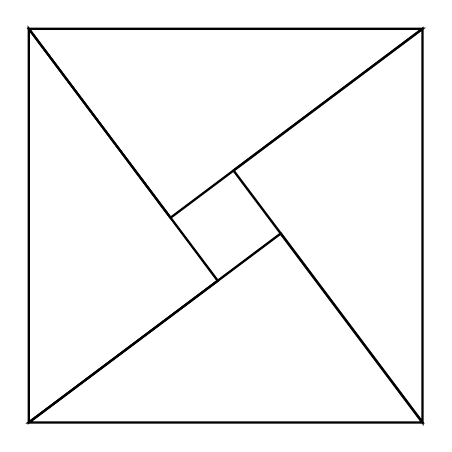
\begin{tikzpicture}
\draw[thick] (0,0) -- (16/5,12/5) -- (5,0) -- cycle;
\draw[thick] (0,0) -- (12/5,9/5) -- (0,5) -- cycle;
\draw[thick] (0,5) -- (5,5) -- (9/5,13/5) -- cycle;
\draw[thick] (5,0) -- (13/5,16/5) -- (5,5) -- cycle;
\end{tikzpicture}
\end{center}
其中四個三角形的短股為$a$、長股為$b$、斜邊為$c$。
\[4\frac{ab}{2}+(b-a)^2=c\]
\[a^2+b^2=c^2\]
\end{proof}
\sssc{三角形全等與$SSA$型性質}
令:已知兩三角形一對應位置之邊長相等稱$S$,已知兩三角形一對應位置之角之角度相等稱$A$,$S$相鄰表示鄰邊,$A$相鄰表示鄰角,$S$與$A$相鄰表示邊與其一側的角,當$A$為直角得稱$R$,$R$之鄰邊得稱$H$。

三角形的全等性質有$SSS$、$SAS$、$AAS$、$ASA$、$RHS$,當兩三角形符合以上任一條件時,知兩三角形全等。

$SSA$型的討論:若已知$a$、$b$、$\angle A$:
\begin{itemize}
\item $\angle A$為銳角,因$C$到$\olra{AB}$的距離為$b\sin A$:
\begin{itemize}
\item $a<b\sin A$: 無解
\item $a=b\sin A$: 唯一解
\item $a>b\sin A$: 兩解
\end{itemize}
\item $\angle A$為鈍角,則:
\begin{itemize}
\item $a\leq b$: 無解
\item $a>b$: 唯一解
\end{itemize}
\end{itemize}
\sssc{九點圓(Nine-point circle)/歐拉圓(Euler's circle)/費爾巴哈圓(Feuerbach circle)與歐拉線(Euler line)}
\bit
\item $M_a,M_b,M_c,h_a,h_b,h_c,\frac{A+H}{2},\frac{B+H}{2},\frac{B+H}{2}$必共圓,該圓稱九點圓(Nine-point circle)、歐拉圓(Euler's circle)或費爾巴哈圓(Feuerbach circle)。
\item 九點圓圓周$\mathscr{O}$與圓心$\mathscr{O}$均符合:
\[\mathscr{O}=\frac{O+H}{2}\]
\item $\mathscr{O},O,G,H$必共線,該線稱歐拉線(Euler line)。
\item $\Delta ABC$ 是等腰三角形 $\iff I$ 在歐拉線上。
\item 費爾巴哈定理(Feuerbach's theorem):九點圓與三個旁切圓均外切,與內切圓內切(內切圓在內)。
\item \[\mathscr{R}=\frac{R}{2}\]
\eit
\sssc{正弦定理(Law of sines)}
\[\frac{\sin A}{a}=\frac{\sin B}{b}\]
\begin{proof}
\[\sin A=\frac{\overline{Ch_c}}{a}\]
\[\sin B=\frac{\overline{Ch_c}}{b}\]
\end{proof}
\[2R\sin A =a\]
\begin{proof}\mbox{}\\
作$O$。若$\Delta ABC$為直角三角形,觀察可證。若$\Delta ABC$非直角三角形,以$BC$為一股,令斜邊在$\olra{BO}$上,作一直角三角形$BCD$,其中$D=2O-B$。若$\Delta ABC$為銳角三角形,根據圓周定理可知,$\angle D = \angle BAC$,得證。若$\Delta ABC$為鈍角三角形,根據根據圓內接四邊形對角互補定理可知,$\angle D = \pi- \angle A$,得證。
\end{proof}
\sssc{凸四邊形面積公式}
\[\text{凸四邊形面積=$\frac{1}{2}$對角線相乘$\times\sin$兩對角線夾角}\]
\sssc{投影定理}
\[a=b\cos C+c\cos B\]
\sssc{餘弦定理(Law of cosines)}
\[a^2=b^2+c^2-2bc\cos A\]
\begin{proof}\mbox{}\\
根據投影定理:
\[c=a\cos B+b\cos A\]
兩邊同乘$c$:
\[c^2=ac\cos B +bc\cos A\]
同理:
\[a^2=ac\cos B +ab\cos C\]
\[c^2=bc\cos A +ab\cos C\]
\[c^2=a^2-ab\cos C+b^{2}-ab\cos C=a^{2}+b^{2}-2ab\cos C\]
\end{proof}
\sssc{平行四邊形邊長與對角線長平方公式}
\[\text{平行四邊形四邊長平方和等於兩對角線長平方和}\]
\sssc{三角形中線公式}
\[\overline{AB}^2+\overline{AC}^2=2\qty(\overline{AM_a}^2+\overline{BM_a}^2)\]
\sssc{三角形面積公式}
\bma
\Delta ABC &= \frac{1}{2}a\cdot \ol{Ah_a}\\
&= \frac{1}{2}ab\sin C\\
&= \sqrt{s(s-a)(s-b)(s-c)}\quad\text{(海龍(Heron)公式)}\\
&= \frac{abc}{4R}\\
&= rs\\
&= \frac{1}{\sqrt{\qty(\frac{1}{h_a}+\frac{1}{h_b}+\frac{1}{h_c})\qty(-\frac{1}{h_a}+\frac{1}{h_b}+\frac{1}{h_c})\qty(\frac{1}{h_a}-\frac{1}{h_b}+\frac{1}{h_c})\qty(\frac{1}{h_a}+\frac{1}{h_b}-\frac{1}{h_c})}}\\
&= \frac{2}{3}\ol{BM_b}\cdot \ol{CM_c}\sqrt{\qty|\frac{1-\qty(\ol{AM_a}^2+\ol{BM_b}^2+\ol{CM_c}^2)^2}{4\ol{BM_b}^2\ol{CM_c}^2}|}\\
&= \frac{1}{2}\sqrt{\ol{AB}^2\ol{AC}^2-\qty(\ora{AB}\cdot \ora{AC})^2}\\
&= \frac{1}{2}\abs{\abs{\ora{AB}\times \ora{AC}}}
\eam
\sssc{重心(Centroid)相關定理}
\[G\tx{\ 為三中線交點}\]
\[\ora{AG}=2\ora{GM_A}\]
\[G=\frac{A+B+C}{3}\]
\[\ora{GA}+\ora{GB}+\ora{GC}=\ora{0}\]
\[\Delta GAB=\Delta GAC=\Delta GBC\]
\sssc{外心(Circumcenter)相關定理}
\[\ol{OA}=\ol{OB}=\ol{OC}=R\]
\[O=\frac{a^2A+b^2B+c^2C}{a^2+b^2+c^2}\]
\[O\tx{\ 為三邊中垂線交點}\]
\[\Delta OAB : \Delta OBC : \Delta OCA = \sin 2C : \sin 2A : \sin 2B\]
\[ \ora{AO}\cdot \ora{AB} = \frac{1}{2}\ol{AB}^2 \]
\[\frac{1}{2}\angle AOB = \angle C\lor\pi -\angle C\]
\sssc{內心(Incenter)相關定理}
\[I\tx{\ 與三邊均相切}\]
\[I\tx{\ 為三角角平分線交點}\]
\[I=\frac{aA+bB+cC}{a+b+c}\]
\[a\ora{IA}+b\ora{IB}+c\ora{IC}=\ora{0}\]
\[\Delta IAB : \Delta IBC : \Delta ICA = c : a : b\]
\sssc{垂心(Orthocenter)相關定理}
\[H\tx{\ 為三高交點}\]
\[H=\frac{\tan A\cdot A+\tan B\cdot B+\tan C\cdot C}{\tan A+\tan B+\tan C}\]
\[ \ora{AH}\cdot\ora{AB}=\ora{AH}\cdot\ora{AC}=\ora{AB}\cdot\ora{AC}=\frac{1}{2}\qty(\ora{AC}^2+\ora{AB}^2-\ora{BC}^2)\]
\[\tx{在複數平面上:}
\det \begin{pmatrix} 1 & A & A^2 & \overline A \\
1& B & B^2 & \overline B \\
1& C & C^2 & \overline C \\
1& H & H^2 & \overline H
\end{pmatrix}=0\]
\[\frac {\overline {Hh_a}}{\overline {Ah_a}}+\frac {\overline {Hh_b}}{\overline {Bh_b}}+\frac {\overline {Hh_c}}{\overline {Ch_c}}=1\]
\sssc{西瓦定理(Ceva theorem)}
令西瓦線段指各頂點與其對邊或對邊延長線連接而成的直線段。
\bma
& \text{三角形$\Delta ABC$的西瓦線段$\ora{AD}$、$\ora{BE}$、$\ora{CF}$:}\\
& \tx{$\ora{AD}$、$\ora{BE}$、$\ora{CF}$ 交於一點} \iff \frac {\overline {BD}}{\overline {DC}}\cdot \frac {\overline {CE}}{\overline {EA}}\cdot \frac {\overline {AF}}{\overline {FB}}=1 \implies D\tx{、}E\tx{、}F\tx{中有零或二個點不在 }\Delta ABC\tx{\ 邊上}
\eam
口訣:頂分頂分頂分頂
\sssc{孟氏定理(Menelaus' theorem)}
\bma
& \text{一直線與${\displaystyle \Delta ABC}$的邊$BC$、$CA$、$AB$或其延長線分別交於$L$、$M$、$N$}\\
& \iff \frac {\overline {AN}}{\overline {NB}}\cdot \frac {\overline {BL}}{\overline {LC}}\cdot \frac {\overline {CM}}{\overline {MA}}=1 \implies L\tx{、}M\tx{、}N\tx{中有一或三個點不在 }\Delta ABC\tx{\ 邊上}
\eam
口訣:頂分頂分頂分頂
\sssc{角平分線定理}
已知:$\Delta ABC$中$\angle B$<$\angle C$;$D$在$\ol{BC}$上;$E$在$\ora{BC}$上且不在$\ol{BC}$上。

內角平分線定理及逆定理:
\[\angle BAD =\angle DAC \Leftrightarrow {\frac {\ol{DB}}{\ol{DC}}}={\frac {\ol{AB}}{\ol{AC}}}\]
外角平分線定理及逆定理:
\[\angle CAE =\pi-\angle BAE \Leftrightarrow {\frac {\ol{EB}}{\ol{EC}}}={\frac {\ol{AB}}{\ol{AC}}}\]
\sssc{角平分線長定理}
\[\ol{A\mathscr{B}_a}=\frac{bc\sin A}{\qty(b+c)\sin\qty(\frac{A}{2})}\]
\ssc{其他圖形公式定理}
\sssc{多邊形內角和公式}
任二邊不相交於該二邊之頂點(如有)以外之處的$n$邊形,其內角和為$(n-2)\pi$。
\sssc{圓內二弦夾角公式}
圓心$O$之圓內二弦$\ol{AB}$、$\ol{CD}$交於$E$,則:
\[\angle AEC=\frac{1}{2}\qty(\angle AOC+\angle BOD)\]
當$B=D=E$:
\[\angle AEC=\frac{1}{2}\angle AOC\]
當$B=D=E$且$\ol{AC}$為一直徑:
\[\angle AEC=\frac{\pi}{2}\]
\sssc{圓內接四邊形公式}
一圓內接四邊形$ABCD$,$\ol{AB}=a$、$\ol{BC}=b$、$\ol{CD}=c$、$\ol{DA}=d$:
\[\angle A+\angle C=\pi\]
\[\ol{AC}^2=\frac{\qty(ac+bd)\qty(ad+bc)}{ab+cd}\]
\[\ol{BD}^2=\frac{\qty(ac+bd)\qty(ad+cd)}{ad+bc}\]
\[\ol{AC}\cdot\ol{BD}=ac+bd\]
\sssc{球面餘弦定律}
空間中與一定點 $O$ 距離為 $R>0$ 的所有點 $P$ 所形成的圖形稱一球面,其中 $O$ 稱為球心,$R$ 稱為半徑。

令球面上有球面三角形$ABC$,$\angle A$之對邊弧長除以球面之半徑等於$a$,$\angle B$之對邊弧長除以球面之半徑等於$b$,$\angle C$之對邊弧長除以球面之半徑等於$c$。

第一球面餘弦定律:
\[\cos c = \cos a \cos b + \sin a \sin b \cos C\]
第二球面餘弦定律/角度餘弦定律:
\[\cos C = - \cos A \cos B + \sin A \sin B \cos c\]
\sssc{四面體內接球半徑定理}
\[\tx{內接球半徑}=\frac{3\cdot\tx{體積}}{\tx{表面積}}\]
\sssc{正四面體各公式}
正四面體A-BCD邊長 $a$,高 $h$,表面積 $A$,體積 $V$,外接球半徑 $R$,內接球半徑 $r$,$\olra{AB}$與$\olra{CD}$距離 $s$,重心 $\frac{A+B+C+D}{4}$與$A$的距離 $g$:
\[h=\frac{\sqrt{6}}{3}a\]
\[A=\sqrt{3}a^2\]
\[V=\frac{\sqrt{2}}{12}a^3\]
\[R=\frac{\sqrt{6}}{4}a\]
\[r=\frac{\sqrt{6}}{12}a\]
\[s=\frac{\sqrt{2}}{2}a\]
\[g=\frac{\sqrt{6}}{4}a\]
\end{document}